\chapter{Evaluation of classification results}
\label{ch:evaluation}

This chapter provides insights into the results after applying the implemented prediction framework described in chapter \ref{ch:dataDriven}. 

The results shown were retrieved by a run finished on the 29.11.2017 at 09:50. Based on the different configurations to generate datasets, the prediction framework finally computed a data set containing 35 features (excluding the class attribute representing the ground truth) whereby 19 features are binary (transformed from nominal ones) and the other 16 are numeric. The data set contained 3082 instances reached by oversampling the minority class with the SMOTE algorithm. It generated 95\% synthetic observations based on the previous number of instances. As a result the new training set contained 1558 instances representing dissatisfied customers and the original 1524 satisfied ones. Regarding missing values, the framework decided to impute all nominal features by the mode of the according feature while missing numeric values were imputed by the mean.  	

Following paragraphs compare the results from the evaluated classifiers with each other. Thereby, a clear differentiation between the two considered types namely, function-based- and rule-based classifiers was done. All following results were retrieved after applying a 10-fold cross validation on the learned model. The first evaluation was done on a support vector machine algorithm based on a polynomial kernel function. Similar to the weak results from the top-down approach, the SVM algorithm turned out to be not able to find an appropriate hyperplane to distinguish between the two classes of satisfied and dissatisfied customers. The results provided showed a weak classification accuracy of only 64.5036\%. The important metrics are summarized in table \ref{tab:svmResults} and will be briefly explained in the following paragraph. 

\begin{table}[]
	\centering
	\begin{tabular}{|l|l|l|l|l|}
		\hline
		\textbf{Classification} & \textbf{True positives} & \textbf{False positives} & \textbf{Precision} & \textbf{ROC Area} \\ \hline
		Dissatisfied            & 0.481                  & 0.188                    & 0.724              & 0.647             \\ \hline
		Satisfied               & 0.812                   & 0.519                    & 0.605                & 0.647             \\ \hline
	\end{tabular}
	\caption{Classification results for support vector machine}
	\label{tab:svmResults}
\end{table}

As very remarkable for the author was the high discrepancy between the true-positive rates although the data set was balanced via SMOTE oversampling before. This prediction weakness can be illustrated quite well with the corresponding visualization of the ROC curve in figure \ref{fig:rocCurveSVM}, showing the relation between true-positives and false-positives regarding classification of satisfied customers. 

\begin{figure}
	\centering
	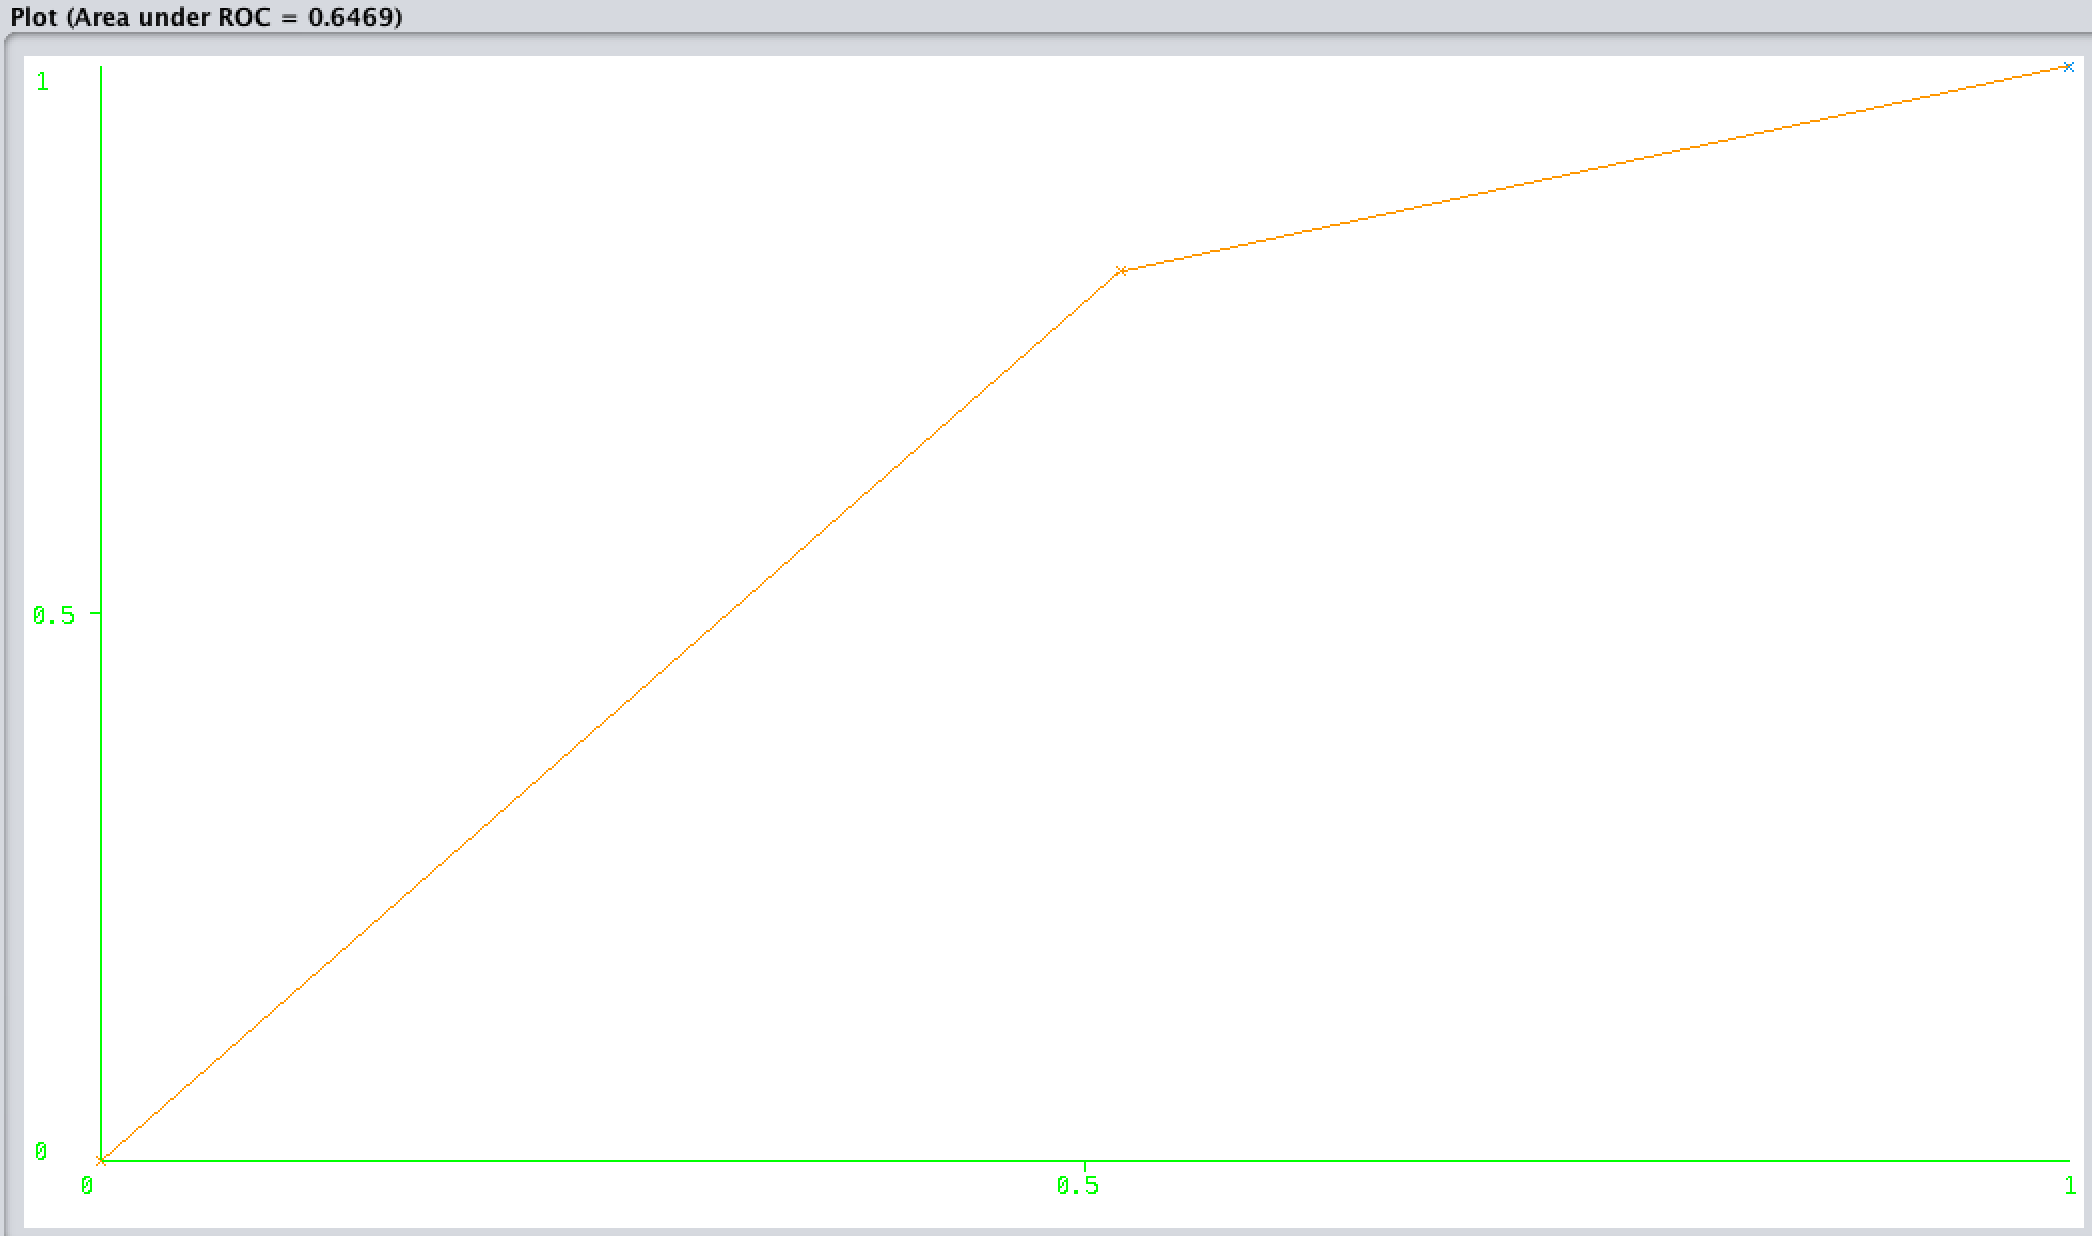
\includegraphics[width=1.0\textwidth]{img/rocResultSVM.png}
	\caption{ROC curve for SVM}
	\label{fig:rocCurveSVM}
\end{figure}

From the perspective of the author it can be followed that the SVM was very vulnerable with regard to the weak correlations of features with the class value and thus did not find any fitting hyperplane function in order to reduce the extremely high false-positive rate from a viewpoint of the satisfied class. 

As outlined in the background research in section \ref{sssec:decisionTrees}, a completely different approach is taken by decision trees where instead of mathematical functions, a rule set of how to split the training data based on the decisive power of features is built. After applying the standard decision tree implementation in Java, namely J48, the overall classification accuracy could increased to 65.7041\%. Moreover the false-positive rates could be stabilized in contrast to the SVM which is a good sign. The detailed metrics are illustrated in table \ref{tab:decisionTreeResult}. 

\begin{table}[]
	\centering
	\begin{tabular}{|l|l|l|l|l|}
		\hline
		\textbf{Classification} & \textbf{True positives} & \textbf{False positives} & \textbf{Precision} & \textbf{ROC Area} \\ \hline
		Dissatisfied            & 0.696                 & 0.383                    & 0.650              & 0.677             \\ \hline
		Satisfied               & 0.617                   & 0.304                    & 0.665                & 0.677             \\ \hline
	\end{tabular}
	\caption{Classification results for J48 decision tree}
	\label{tab:decisionTreeResult}
\end{table}

Although a decision tree can be considered as rather simple classification technique, it seems to fit the data set used in the case study of this thesis much better than the SVM. Moreover, learning the model is much faster as well. However, from an objective perspective the results are still not expressive as they are far too error prone and do not allow for a reliable prediction. As a result the framework decided also evaluated the decision tree variant called Random forest which was introduced in section \ref{sssec:decisionTrees}. 

The evaluation results of the Random forest algorithm showed major improvements in contrast to the standard decision tree and SVM algorithm. The basic configuration used for the random forest constructed 100 decision trees. For the preprocessed data set adhering the described configuration, a classification accuracy of 75.146 \% could be achieved. Although this was the highest accuracy achieved, the AUC value indicating the area under ROC curve is worse than the evaluation with a cost sensitive meta classifier. As mentioned in the literature research, depending on the task the classification accuracy is not expressive enough. Since from a business perspective correctly detecting dissatisfied customers is essential, the number of false negatives should be as low as possible even though it sacrifices the false positives. As a consequence the appropriate choice taken by the author was to penalize false negative classifications with a cost of 1.5. This way the true positive rate with regard to dissatisfied customers could be established on an acceptable level. Due to this change the according false positive rate increased accordingly. Table \ref{tab:classificationResults} shows a summary of the important measurement results.

\begin{table}[]
	\centering
	\begin{tabular}{|l|l|l|l|l|}
		\hline
		\textbf{Classification} & \textbf{True positives} & \textbf{False positives} & \textbf{Precision} & \textbf{ROC Area} \\ \hline
		Dissatisfied            & 0.847                   & 0.375                    & 0.698              & 0.847             \\ \hline
		Satisfied               & 0.625                   & 0.153                    & 0.8                & 0.625             \\ \hline
	\end{tabular}
 	\caption{Classification results for Cost-sensitive Random forest}
 	\label{tab:classificationResults}
 \end{table}

The corresponding ROC curve is shown in figure \ref{fig:rocCurve}. 

\begin{figure}
	\centering
	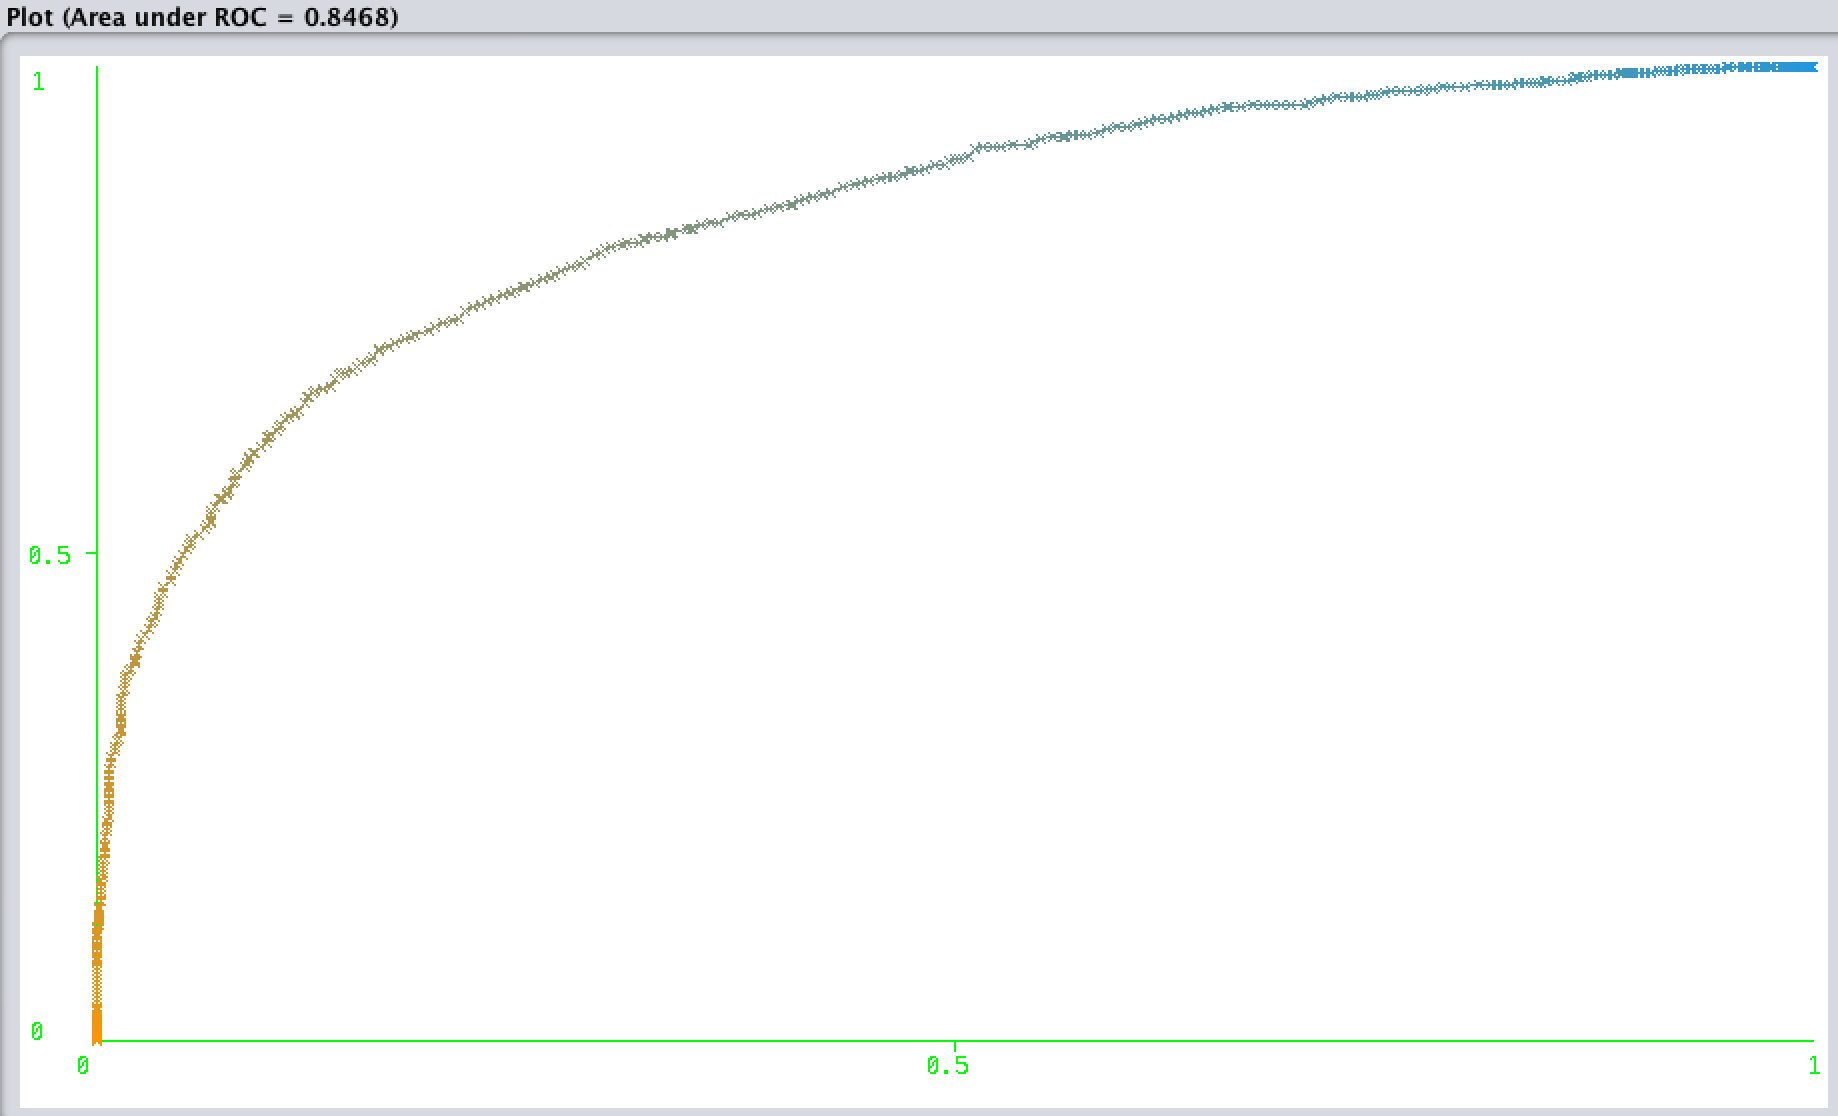
\includegraphics[width=1.0\textwidth]{img/rocResultRF.png}
	\caption{ROC curve for Cost-Sensitive Random Forest}
	\label{fig:rocCurve}
\end{figure}

In order to verify how powerful the built model which produced the results from table \ref{tab:classificationResults} is, it was validated against a test set not included in the training phase. This should check whether and to which extent the model is vulnerable to the overfitting phenomenon, i.e. how good the classification accuracy can be expected on a real production data set. Therefore the full training set, which was used for cross-validation during the training phase, was split randomly into two separate files. The new training set contained 80\% while the test set consisted of the remaining 20\%. This approach was done manually via the Weka Explorer using the Resample filter. After loading the new training set and the trained model from the previous step into the Weka Explorer, the evaluation could be done against the provided test set. The results showed a slightly diminished overall accuracy of 70.928\%. Table \ref{tab:testResults} shows again a more detailed overview on the important metrics.

\begin{table}[]
	\centering
	\begin{tabular}{|l|l|l|l|l|}
		\hline
		\textbf{Classification} & \textbf{True positives} & \textbf{False positives} & \textbf{Precision} & \textbf{ROC Area} \\ \hline
		Dissatisfied            & 0.779                   & 0.354                    & 0.667              & 0.804             \\ \hline
		Satisfied               & 0.646                   & 0.221                    & 0.763                & 0.804             \\ \hline
	\end{tabular}
	\caption{Classification results for Cost-sensitive Random forest evaluated on supplied test set}
	\label{tab:testResults}
\end{table}

Analyzing the results of the prediction framework led to following technical findings. Firstly, decision trees as base classifier and especially the ensemble algorithm Random Forest outperformed the Support Vector machines. Thus it can be followed that a rule-based classification approach suits the prediction of Customer Satisfaction based on usage features better than a functional approach like SVM. Regarding preprocessing and transformation of the data set, oversampling drastically improved the performance of the classifier. Generated data sets in the preprocessing phase which did not deal with the class imbalance explicitly, produced very bad results due to the reason that the given classification algorithm favored the class of satisfied customers which caused far too many false-positives. This shifted attention of the author to an intensive research and experimenting phase to tackle the class imbalance problem whereby the SMOTE algorithm finally turned out to be well suited since it could keep the performance in training high but did not overfit the trained model too much. Quite some effort was put on finding a preferred method to handle missing data. Although in the literature, mean and mode imputation were sometimes criticized to introduce bias in the data and thus diminish power of classification, the prediction framework selected the rather simple but broadly used method when achieving the best results. This was a bit surprising to the author as the k-nearest neighbor implementation was considered as more sophisticated and also yielded better results in dedicated research experiments as outlined for instance in \cite{batista2003analysis}.

The following final chapter will conclude the thesis by wrapping up the work done in this research. Furthermore it draws consequences based on the findings and provides a look into future work. 